%
% LaTeX template for Dual Degree / Masters thesis at IITB
%
% Created by Neehar Jathar
%
% The official requirement has been persisted with, even if some things could look better some other way.
% Tamper with any of the settings as you see fit and, more importantly, as your guide sees fit.
% Most sections have comments. A lot of stuff is explained in Chapter 1 regarding how to use this template.
% Code snippets for inserting figures, tables and equations are also there in Chapter 1
% Hopefully, this will make report making a little easier.
%

% OK. Here goes.

% Preamble

% Official font size is 12. I thought 11 looked better.
% A4 paper size
% Template for one sided printing of the thesis
\documentclass[12pt, a4paper, oneside]{book}

% Set of packages included. These are all the packages I required, maybe some would be unnecessary and some might be missing. 
% Add any new packages you use over here.

\usepackage[utf8]{inputenc}
\usepackage{setspace}
\usepackage{amsmath,amsfonts,amssymb,amscd,amsthm,xspace}
\usepackage{titlesec}
\usepackage{vmargin}
\usepackage{fancyhdr}
\usepackage{caption}
\usepackage{subcaption}
\usepackage{multirow}
\usepackage{multicol}
\usepackage{url}
\usepackage{tabularx}
\usepackage{graphicx}
\usepackage{epstopdf}
\usepackage{booktabs}
\usepackage{rotating}
\usepackage{listings}
%\usepackage[centerlast,small,sc]{caption}
\usepackage[square, numbers, comma, sort&compress]{natbib} % Standard reference style with [3], [4] type numbers in the text and entries sorted according to order of appearance in the References
\usepackage[pdfpagemode={UseOutlines},bookmarks=true,bookmarksopen=true,bookmarksopenlevel=0,bookmarksnumbered=true,hypertexnames=false,colorlinks,linkcolor={black},citecolor={black},urlcolor={black},pdfstartview={FitV},unicode,breaklinks=true]{hyperref}
\hypersetup{urlcolor=black, colorlinks=true} % colors hyperlinks in blue - change to black if annoying

% Math operator definition - may not be required
% If any new operators are required, defien them here
\DeclareMathOperator*{\argmin}{argmin}

\title{\thesisTitle}
\author{\authorName}
\date{\today}

% Currently chapter title has been centered, to left align the chapter title and number, change \centering to \flushleft
\titleformat{\chapter}[display]
  {\normalfont\huge\bfseries\centering}
  {\chaptertitlename\ \thechapter}{18pt}{\Huge}

\setmarginsrb   { 3.0cm}  % left margin
                { 1.5cm}  % top margin
                { 2.0cm}  % right margin
                { 2.2cm}  % bottom margin
                { 0.3cm}  % head height
                { 1.2cm}  % head sep
                { 0.3pt}  % foot height
                { 1.0cm}  % foot sep

% End of the Preamble

% Actual document begins
\begin{document}

\newcommand{\HRule}{\rule{\linewidth}{0.5mm}} % New command to make the lines in the title page

% Import all the variable values from Details.tex
% This file contains all the user specific things that need to be changed such as the thesis title, author name etc. 


\newcommand{\thesisTitle}{Implementation of LDPC Decoder Using AHIR Tool Chain }

\newcommand{\degree}{Master of Technology}

\newcommand{\authorName}{Anurag Gupta}

\newcommand{\rollNo}{153070050}

\newcommand{\dept}{Department of Electrical Engineering}

\newcommand{\college}{Indian Institute of Technology Bombay}

\newcommand{\currentyear}{2017}

\newcommand{\currentmonth}{June}

\newcommand{\supervisorOne}{Prof. Madhav P. Desai}

\newcommand{\supervisorTwo}{Prof. Supervisor Two}

\newcommand{\examinerOne}{Prof. Examiner One}

\newcommand{\examinerTwo}{Prof. Examiner Two}

\newcommand{\chairman}{Prof. Chairman}


% Use roman page numbering style (i, ii, iii, iv...) for the pre-content pages
\frontmatter

% Line spacing of 1.5 as per IIT requirement. If you think it looks too spaced out, use 1.3
% I think 11 pt font with 1.3 spacing looks quite good
\setstretch{1.5}

% Import all the pages in the front matter
% This file contains the templates for the first few pages of the thesis including 
% 1. Title page
% 2. Dedication
% 3. Dissertation approval
% 4. Declaration of authorship
% 5. Abstract


%   1. TITLE
\newcommand{\titlePage}{

% No page number
\thispagestyle{empty}
\begin{center}

% thesis title
\vspace*{15px}
{\Huge\bfseries \thesisTitle}\\[1.0cm] 

% submitted in partial fulfillment etc.
\textit{Submitted in partial fulfillment of the requirements\\[0.2cm] of the degree of\\[0.2cm] \degree}\\[2.0cm]
 
% author
\textit{by}\\[0.2cm]
\authorName \\[0.2cm] (\textit{Roll no.} \rollNo) \\[2.0cm]

% supervisor
\textit{Supervisor:}\\[0.2cm]
% or
% \textit{under the supervision of}\\[0.2cm]
\supervisorOne \\[2.0cm]

% iit-b logo

\includegraphics[width=0.25\textwidth]{Figures/iitb_logo.jpg}

\vspace*{10px}

% department and college
\dept\\[0.2cm]
\college\\[0.2cm]

% year
\currentyear\\[4cm] 

\end{center}

\clearpage
}

%   2. DEDICATION
\newcommand{\dedication}{
\thispagestyle{empty}
\vspace*{75px}
\begin{center}\large{\textit{Dedicated to ...}}\end{center}

\clearpage
}

%   3. DISSERTATION APPROVAL

\newcommand{\approval}{
% if you use a dedication, then use a page number with the plain page style
\thispagestyle{plain}
% else, use no page number with the empty page style
%\thispagestyle{empty}


% page title
\begin{center}{\huge\bf Dissertation Approval\par}\end{center}

\vspace*{15px}

\noindent This dissertation entitled 
% title
\textbf{``\thesisTitle"}, submitted by 
% author
\authorName  
(Roll No.  \rollNo),
is approved for the award of degree of 
% degree
\degree 
in 
% branch
XYZ Engineering.\\[1.0cm]

% examiners and supervisors
\begin{flushright}
\textbf{{Examiners}}\\[0.8cm]
\examinerOne\quad\rule{0.3\textwidth}{.3pt}\\[0.8cm]
\examinerTwo\quad\rule{0.3\textwidth}{.3pt}\\[1.6cm]

\textbf{{Supervisor}}\\[0.8cm]
\supervisorOne \quad\rule{0.3\textwidth}{.3pt}\\[1.6cm]

\textbf{{Chairman}}\\[0.8cm]
\chairman\quad\rule{0.3\textwidth}{.3pt}\\[2.4cm]

\end{flushright}
\textbf{Date:} ...... \currentmonth { } \currentyear\\[0.3cm]
\textbf{Place:}\quad\rule{0.5\textwidth}{.3pt} 

% start a new page
\clearpage
}

%   4. DECLARATION OF AUTHORSHIP
\newcommand{\authorship}{
\thispagestyle{plain}

\begin{center}{\huge\bf Declaration of Authorship\par}\end{center}

\vspace*{15px}

% institute declaration text
\noindent I declare that this written submission represents my ideas in my own words and where others' ideas or words have been included, I have adequately cited and referenced the original sources.  I also declare that I have adhered to all principles of academic honesty and integrity and   have   not   misrepresented   or   fabricated   or   falsified   any   idea/data/fact/source   in   my submission.  I understand that any violation of the above will be cause for disciplinary action by the Institute and can also evoke  penal action from the sources which have thus not been properly cited or from whom proper permission has not been taken when needed.

\vspace*{10px}

% signature
\begin{flushright}
{Signature: ......................................\\[0.4cm]}

% author name
{\textbf{\authorName}\\[0.0cm]\rollNo\\[2.0cm]}

\end{flushright}
% date
\begin{flushleft}
{Date: ...... \currentmonth { } \currentyear\\}
\end{flushleft}


% start a new page
\clearpage 
}

%   5. ABSTRACT
\newcommand{\abstractpage}{
\thispagestyle{plain}

% header-type text for the abstract - optional
\small {\noindent\authorName/ \supervisorOne{ }(Supervisor): \textbf{``\thesisTitle"}, \textit{Dual Degree Dissertation}, \dept, \college, \currentmonth { } \currentyear.}\\[0.0cm]
\HRule\\[0.2cm]


\vspace*{10px}

\begin{center}{\huge{\textit {Abstract}}\par}\end{center}

\vspace*{10px}

% Abstract text - Type abstract here
\noindent Enter Abstract text here, in the file TheFrontMatter.tex \\[0.2cm]

% Index terms
\noindent \textbf{Index terms:} 

% Start a new page
\clearpage 
}


\titlePage

\setcounter{page}{1}
\dedication

\addcontentsline{toc}{chapter}{Dissertation Approval}
\approval

\addcontentsline{toc}{chapter}{Declaration of Authorship}
\authorship

\addcontentsline{toc}{chapter}{Abstract}
\abstractpage

\pagestyle{fancy}

% Set the left side page header to "Contents"
\lhead{\emph{Contents}} 

% Write out the Table of Contents
\tableofcontents 

% Set the left side page header to "List of Figures"
\lhead{\emph{List of Figures}} 

% Write out the List of Figures
\listoffigures 
\addcontentsline{toc}{chapter}{List of Figures}

% Set the left side page header to "List of Tables"
\lhead{\emph{List of Tables}} 

% Write out the List of Tables
\listoftables
\addcontentsline{toc}{chapter}{List of Tables}

\fancyhead{}
\rhead{\thepage}


% Use arabic page numbering style (1, 2, 3...) for the body of the report
\mainmatter

% Import the Chapters
% Introduction

% Main chapter title
\chapter{Introduction} 
% Change X to a consecutive number; for referencing this chapter elsewhere, use \ref{ChapterX}
\label{Chapter1} 
% This is for the header on each page
\lhead{Chapter 1. \emph{Introduction}}


\section{Motivation }
The error performance of the low density parity check  codes approach to Shannon limit, which make low density parity check code the best known codes. An active research is going on to implement the low density parity check decoder for storage devices to achieve the bit error rate of the order of $10^{-16}$. Thus, to make a low density parity check  decoder with a optimum cost and performance trade off is a challenging task.

\section{Organisation of the Report }

In chapter 1, we have discussed the basics of error correction in a communication channel. In chapter 2, we have discussed how to generate different parity check matrices. In chapter 3, we have discussed different decoding algorithms in detail. In chapter 4, we have shown the results of the C level implementation of Min Sum decoding algorithm. In chapter 5, we have discussed the concept and procedure to partition a parity check matrix. Level of parallelism is taken as a metric and results are plotted and discussed. In chapter 6, we have deployed partitioning in the matrix and modified the decoding algorithm to parallelise the hardware. In chapter 7, the conversion of the algorithms from C to VHDL is discussed along with results of the implementation of the algorithm on FPGA.
\section{Basics of Error Correction }
  
The goal of communication is to transmit a message and receive it correctly even after noisy transmission through the channel. This is achieved by introducing redundancy in the message at the transmitter side, called as encoding of message. The encoded message is called codeword. Then codeword is then transmitted through the noisy channel, which alters the codeword. By some error correcting algorithm the message is extracted back at receiver side, called decoding of the codeword. Thus, the error free transmission takes place by applying error correcting codes in communication system.\\
We have a k bit long message. To encode it we introduce m redundant bits (called parity bits) to form an $n(=m+k)$ bit long codeword. This category of codes are called (n,k) block codes. 

\subsection{Parity Check Matrix}

The codeword must satisfy a group of conditions to ensure error free transmission or to indicate the error has taken place. If error occurs, the error can be corrected by applying some algorithm on those group of conditions . The group of conditions are called parity check equations.The matrix form of the condition is called parity check matrix. \\
Example: If a code block $y=[c_1\, c_2\,c_3\, c_4\, c_5\, c_6]$ has to satisfy following parity check equations. 
\begin{align}
c_1 \oplus c_2 \oplus c_4 =0 \\
 c_2 \oplus c_3 \oplus c_5 =0 \\
c_1 \oplus c_2 \oplus c_3 \oplus c_6 =0 
\end{align}  
Then it's parity check matrix is as follows:
\begin{align}
 H= \left[ \begin{array}{cccccc}
1 & 1 & 0 & 1 & 0 & 0\\
0 & 1 & 1 & 0 & 1 & 0\\
1 & 0 & 0 & 0 & 1 & 1\\
0 & 0 & 1 & 1 & 0 & 1  
\end{array} \right]  
\end{align} 
s.t. $Hy^T=0$.

\subsection{Encoding of Message}
We can rewrite the above equations (1),(2),(3) as:
\begin{align}
c_4 = c_1 \oplus c_2 \\
c_5 = c_2 \oplus c_3 \\
c_6 = c_1 \oplus c_2 \oplus c_3  
\end{align}  
We can find parity check bits $c_4,c_5,c_6$ by message bits $c_1,c_2,c_3$.
Thus we can encode message bits to find codeword. \\
Encoding is preferably done in matrix form, by manipulating parity check matrix to find a generator matrix.
If parity check matrix can be written in the form
$H = [A, I_{n- k} ]$,
where A is an $(n-k)$xk binary matrix and $I_{n-k}$ is the identity matrix of order
$(n-k)$. The generator matrix is then
$G = [I_k , A^T ]$.
s.t $GH^T = 0$. \\
\begin{align}
[c_1 c_2 ... c_6]=[c_1 c_2 c_3] \left[ \begin{array}{cccccc}
1 & 0 & 0 & 1 & 0 & 1\\
0 & 1 & 0 & 1 & 1 & 1\\
0 & 0 & 1 & 0 & 1 & 1  
\end{array} \right]
\end{align}
 

Thus, if m is message block containing message bits $[c_1 c_2 c_3]$, then codeword can be generated as $y=mG$.

\subsection{Transmission of the Code Block}
The code block is then transferred through a noisy communication channel that corrupts the code block. According to the behaviour of the noise that is added to the code block, various models of communication channels exists. 
\subsubsection{Binary Symmetric Channel}
 As the name suggests the channel is binary, it has two input symbols and two output symbols. The channel is symmetric because the probability of receiving 0 when 1 was send is same as probability of receiving 1 when 0 was sent. The error probability is also called cross over probability. The transition probability diagram is shown in figure \ref{bsc}
 \begin{figure}[h]
\centering
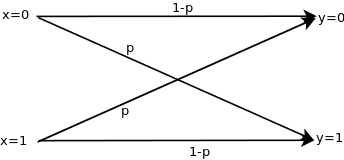
\includegraphics[height=6cm,width=12cm]{bsc}
\caption[Transition probability diagram of Binary Symmetric Channel]{Binary Symmetric Channel}
\label{bsc}
\end{figure}
The cross over probability is denoted as p.
\begin{align} p(y=0|x=1) = p(y=1|x=0) = p  \end{align}
\begin{align} p(y=1|x=1) = p(y=0|x=0) = 1-p  \end{align}
\subsubsection{AWGN (A White Gaussian Noise Channel)}
If a signal in a digital system is represented a continuous random variable as,
\begin{align} Y = X + Z \end{align}
where X is the digital information carrier and Z is the noise component then we can define a Gaussian channel that has input X and output Y, with noise as a Gaussian random variable Z. \\
The pdf of a Gaussian random variable is expressed as follows: \\
\begin{align} f_y(x) = \dfrac{1}{\sqrt{2\pi\sigma^{2}}} \exp{\dfrac{-(x-m)^2}{2\sigma^2}}
 \end{align} 
where m is mean and sigma is standard deviation of the random variable Z.
\subsection{Error Detection \& Correction}

If the codeword gets corrupted in the transmission then all the parity check equations will not get satisfied. Thus, we will get $Hy^T\neq0$. The non-zero vector is called syndrome. That shows that received message is corrupted. But there is a certain limit to the number of bits upto that error can be detected and corrected.
The limit is represented in term of hamming distance. Hamming distance between two codes is number of flipped bits between them. If $d_{min}$ is minimum distance between codes then maximum number of bits upto which error can be correctly detected is $d_{min}-1$ and maximum number of bits upto which error can be corrected is
(t) = $[\frac{d_{min}-1}{2}]$
where [] denotes greatest integer function.\\
More the number of redundant bits, more is the hamming distance. Thus, more error bits can be detected and corrected but the code rate is reduced. The correction is done by directly taking the received vector and comparing it to all the codewords and correcting it to the codeword having minimum distance to it. This is called maximum likelihood decoding. But if n is larger then this task becomes complex. LDPC maximum likelihood decoding, bit flipping decoding are other decoding schemes which reduce complexity of this task.










%% Introduction

% Main chapter title
%\chapter{Theory of LDPC} 

% Change X to a consecutive number; for referencing this chapter elsewhere, use \ref{ChapterX}
%\label{Chapter2} 

% This is for the header on each page
%\lhead{Chapter 2. \emph{Theory of LDPC}}  

The goal of communication is to transmit a message and receive it correctly even after noisy transmission through the channel. This is achieved by introducing redundancy in the message at the transmitter side, called as encoding of message. The encoded message is called codeword. Then codeword is then transmitted through the noisy channel, which alters the codeword. By some error correcting algorithm the message is extracted back at receiver side, called decoding of the codeword. Thus, the error free transmission takes place by applying error correcting codes in communication system.\\
We have a k bit long message to encode it we introduce a m bit redundancy (or called parity bits) to form a $n(=m+k)$ bit long codeword. These category of codes are called (n,k) block codes. 

\subsection{Parity Check Matrix}

The codeword must satisfy a group conditions to ensure error free transmission or to indicate the error have been taken place. If error occurs, the error can be corrected by applying some algorithm on those group of conditions . The group of conditions are called parity check equations.The matrix form of the condition is called parity check matrix. \\
Example: If a code block $y=[c_1 c_2 c_3 c_4 c_5 c_6]$ has to satisfy following parity check equations. 
\begin{align}
c_1 \oplus c_2 \oplus c_4 =0 \\
 c_2 \oplus c_3 \oplus c_5 =0 \\
c_1 \oplus c_2 \oplus c_3 \oplus c_6 =0 
\end{align}  
Then it's parity check matrix is as follows:
\begin{align}
 H= \left[ \begin{array}{cccccc}
1 & 1 & 0 & 1 & 0 & 0\\
0 & 1 & 1 & 0 & 1 & 0\\
1 & 0 & 0 & 0 & 1 & 1\\
0 & 0 & 1 & 1 & 0 & 1  
\end{array} \right]  
\end{align} 
s.t. $Hy^T=0$.

\subsection{Encoding of Message}
We can rewrite the above equations (1),(2),(3) as:
\begin{align}
c_4 = c_1 \oplus c_2 \\
c_5 = c_2 \oplus c_3 \\
c_6 = c_1 \oplus c_2 \oplus c_3  
\end{align}  
We can find parity check bits $c_4,c_5,c_6$ by message bits $c_1,c_2,c_3$.
Thus we can encode message bits to find codeword. \\
Encoding is preferably done in matrix form, by manipulating parity check matrix to find a generator matrix.
If parity check matrix can be written in the form
$H = [A, I_{n- k} ]$,
where A is an $(n-k)$xk binary matrix and $I_{n-k}$ is the identity matrix of order
$(n-k)$. The generator matrix is then
$G = [I_k , A^T ]$.
s.t $GH^T = 0$. \\
\begin{align}
[c_1 c_2 ... c_6]=[c_1 c_2 c_3] \left[ \begin{array}{cccccc}
1 & 0 & 0 & 1 & 0 & 1\\
0 & 1 & 0 & 1 & 1 & 1\\
0 & 0 & 1 & 0 & 1 & 1  
\end{array} \right]
\end{align}
 

Thus, m is message block containing message bits $[c_1 c_2 c_3]$, then codeword can be generated as $y=mG$.

\subsection{Error Detection \& Correction}

If the codeword got corrupted in the transmission then all the parity check equation will not get satisfied. This we will get $Hy^T\neq0$. The non-zero vector is called syndrome. That shows that received message is corrupted. But there is a certain limit in number of bits upto that error can be detected and corrected.
The limit is represented in term of hamming distance. Hamming distance between two codes is number of flipped bits between them. If $d_{min}$ is minimum distance between codes then maximum number bit flipped to which error can be correctly detected is $d_{min}-1$ and maximum number of bits upto which error can be corrected is
(t) = $[\frac{d_{min}-1}{2}]$
where [] denotes greatest integer function.\\
The more the number of redundant bits the more the hamming distance thus more error bits can be detected and corrected but the code rate is reduces. The correction is directly taking the received vector and comparing it to all the codewords and correcting it to the codeword having minimum distance to it. This is called maximum likelihood decoding. But if n is lager then this task become complex. LDPC maximum likelihood decoding, bit flipping decoding are other decoding schemes which reduce complexity of this task.









%% Introduction

% Main chapter title
\chapter{Generation of different LDPC matrices} 

% Change X to a consecutive number; for referencing this chapter elsewhere, use \ref{ChapterX}
\label{Chapter2} 

% This is for the header on each page
\lhead{Chapter 2. \emph{Generation of different LDPC matrices}}  

The Bit Error Rate of decoded code word depends upon properties of parity check matrix. A good parity check matrix should be sparse and  it should have good girth.  

Basic parameters to decide the formation of parity check matrix are as follows . 
\begin{itemize}
\item  \textbf{Random parity check matrix vs systematic parity check matrix:} Parity check matrix that has a specific method of filling $1s$ in matrix is called systematic parity check matrix, else if the position of $1s$ is random, the matrix is called random parity check matrix.
\item\textbf{Regular parity check matrix vs irregular parity check matrix:} Regular parity check matrix has constant number of $1s$ in row and columns, whereas irregular parity check matrix has variable number of $1s$ in its rows and columns. \\
	If $w_c$ is number of $1s$ in a column and $w_r $ is number of $1s$ in a row then in a m$\times$ n regular parity check matrix
\begin{align}
 m * ( w_r ) = n * ( w_c )  
\end{align}
%Collectively the set
%v and h is called the degree distribution of the code. 
%\item columns are divided in $w_r$ sets n/$w_r$ columns in each set. 
If we take the fraction of columns
of weight i by $v_i$ and the fraction of rows of weight i by $h_i$ then in a irregular parity check matrix
\begin{align} m * \sum_{i} (h_i*i) = n *\sum_{i} (v_i*i) 
\end{align}


\end{itemize} 
%\renewcommand{\labelitemi}{$\square$}
\section{Gallager Parity Check Matrix}
Gallager proposed parity check matrix is regular in nature\cite{1}. A regular matrix has constant number of non-zero entries in a row and a column. 
These are represented as (n,$w_c$,$w_r$) codes. where,
\\
$w_c$ = Number of 1\textsuperscript{'}s in a column 
\\
$w_r$ = Number of 1\textsuperscript{'}s in a row 
\\
n = Block length. \\
\textbf{Method of construction:} \\
\noindent o Divide rows in $w_c$ sets with ( m / $w_c$ ) rows in each set.  \\
%\item columns are divided in $w_r$ sets n/$w_r$ columns in each set. 
o All rows of first set of rows contain $w_r$ consecutive once ordered from left to right. \\
o Every other set of rows is random column permutation of first set of rows. \\
\textbf{Example of Gallager Matrix:} \\
( n , $w_c$ , $w_r$ ) = ( 12 , 3 , 4 ) ; m = 9 
\[
 H=
 \left[ \begin{array}{cccccccccccc}
1 &  1 &  1  & 1 &  0 & 0 & 0 & 0 & 0 & 0 & 0 & 0 \\
0 & 0 & 0 & 0 & 1 &  1 &  1  & 1 & 0 & 0 & 0 & 0 \\
0 & 0 & 0 & 0 & 0 & 0 & 0 & 0 & 1 &  1 &  1  & 1 \\
-& - & - & - & - & - & - & - & - &  - &  -  & -\\ 
1 &  0 &  1  & 0 &  0 & 1 & 0 & 0 & 0 & 1 & 0 & 0 \\
0 & 1 & 0 & 0 & 0 &  0 &  1  & 1 & 0 & 0 & 0 & 1 \\
0 & 0 & 0 & 1 & 1 & 0 & 0 & 0 & 1 &  0 &  1  &  0\\
-& - & - & - & - & - & - & - & - &  - &  -  & -\\ 
1 & 0 & 0 & 1 & 0 & 0 & 1 & 0 & 0 & 1 & 0 & 0 \\
0 & 1 & 0 & 0 & 0 & 1 & 0 & 1 & 0 & 0 & 1 & 0 \\
0 & 0 & 1 & 0 & 1 & 0 & 0 & 0 & 1 & 0 & 0 & 1 \\ \end{array} \right]  
\]


\section{Quasi-Cyclic (QC) parity Check Matrix}
QC matrix can be constructed by 
Sridhara Fuja Tanner (SFT)\cite{3} method is discussed. Performance of quasi-cyclic codes is better for smaller block length, comparable for moderate block length with respect to random-regular codes.\\
Method of Construction of (j,k)-regular QC-LDPC code:
\begin{itemize}
\item Construct two sequences $\{s_1,s_2,...,s_{j-1}\}$ and $\{t_1,t_2,...,t_{k-1}\}$, whose elements are randomly selected from GF(p), where p is prime and p$>$2 , $s_i \neq s_x \ \& \ t_i \neq t_x$ if i $\neq$x.
\item Now, form a preliminary matrix Y with the elements of GF(p) as follows:
\begin{align}
 E= \left[ \begin{array}{cccc}
e_{0,0} & e_{0,1} & \cdots & e_{0,k-1} \\
e_{1,0} & e_{0,1} & \cdots & e_{0,k-1} \\
\vdots & \vdots & \ddots & \vdots \\
e_{j-1,0} & e_{j-1,1} & \cdots & e_{j-1,k-1} 
\end{array} \right] 
\end{align}
 
where (i,j)th element of E is calculated by following quadratic congruential equation for a fix parameter
$\kappa\epsilon\{1,2,...,p-1\} $ and $\nu_i,\nu_j\epsilon\{1,2,...,p-1\} $: 
\begin{align}
 e_{i,j}=[\kappa(s_i+t_j)^2 + \nu_i +\nu_j] 
\end{align}
\item So the parity check matrix H is represented by jXk array of circulant permutation of identity matrix. 
\[
 H= \left[ \begin{array}{cccc}
I(e_{0,0}) & I(e_{0,1}) & \cdots & I(e_{0,k-1}) \\
I(e_{1,0}) & I(e_{0,1}) & \cdots & I(e_{0,k-1}) \\
\vdots & \vdots & \ddots & \vdots \\
I(e_{j-1,0}) & I(e_{j-1,1}) & \cdots & I(e_{j-1,k-1}) 
\end{array} \right] \]

 
Where I(x) is p$\times$p identity matrix with row cyclically shifted right by x position.
\end{itemize}

\section{MacKay Neal Parity Check Matrix}
Mckey Neal proposed regular (n,$w_c$,$w_r$) construction of codes using random distribution of non-zero entries\cite{2}. These codes have better performance for large block length compared to other codes.
Method of construction:
\begin{itemize} 
\item Start from the first column. Place $w_c$ 1s in the column randomly and track number of 1s in a row.
\item Repeat the process for other columns. Break only if at any point number of 1\textsuperscript{'}s in the row becomes greater than $w_r$.
\item If break occurs then go back to some columns and repeat algorithm till all columns get filled.
\end{itemize} 
\textbf{Example:}\\
 n = 12, m = 9  
  \[H=
 \left[ \begin{array}{cccccccccccc}
1 & 0 & 0 & 0 & 0 & 1 & 0 & 1 & 0 & 1 & 0 & 0 \\
1 & 0 & 0 & 1 & 1 & 0 & 0 & 0 & 0 & 0 & 1 & 0 \\
0 & 1 & 0 & 0 & 1 & 0 & 1 & 0 & 1 & 0 & 0 & 0 \\
0 & 0 & 1 & 0 & 0 & 1 & 0 & 0 & 0 & 0 & 1 & 1 \\
0 & 0 & 1 & 0 & 0 & 0 & 1 & 1 & 0 & 0 & 0 & 1 \\
0 & 1 & 0 & 0 & 1 & 0 & 0 & 0 & 1 & 0 & 1 & 0\\
1 & 0 & 0 & 1 & 0 & 0 & 1 & 0 & 0 & 1 & 0 & 0 \\
0 & 1 & 0 & 0 & 0 & 1 & 0 & 1 & 0 & 1 & 0 & 0 \\
0 & 0 & 1 & 1 & 0 & 0 & 0 & 0 & 1 & 0 & 0 & 1 \\ \end{array} \right]  
\] 

MacKay Neal construction can be adapted to avoid cycles of length 4, called 4-cycles.\\
Method to avoid 4-cycles\cite{7}:
\begin{itemize}
\item First, generate a preliminary parity check matrix.
\item Put 1s to parity check matrix in rows that don't have any 1s in them or that have only one 1. The places where 1s are to be added in those rows are selected randomly. 
\item Choose odd number of 1s to put in a column. If preliminary parity check matrix constructed has an even number of 1s in each column, problem may occur that will cause the rows to sum up to zero, and hence at least one check will become redundant.
\item To remove situation that has a pair of columns both have all 1s in a particular pair of rows, that makes cycles of length four in graph, one of the 1s involved is moved randomly within its column.
\end{itemize}
Eliminating the cycles improves the girth of the graph and thus improves the convergence and make the iterative decoding faster.  
%%%%%%%%%%%%%%%%%%%%%%%%%%%%%%%%%%%%%%%%%%%%%%%%%%

%% Introduction

% Main chapter title
\chapter{Decoding Algorithm} 

% Change X to a consecutive number; for referencing this chapter elsewhere, use \ref{ChapterX}
\label{Chapter3} 

% This is for the header on each page
\lhead{Chapter 3. \emph{Decoding Algorithms}}  

\section{Message Passing Decoding}


The algorithms used to decode LDPC codes are iterative in nature. In every iteration some information has to be passed through the edge of the bipartite graph (Tanner graph), representing corresponding parity check matrix. Thus these type of iterative algorithm are generally termed as message passing decoding\cite{9}.\\

An equivalent representation of a LDPC parity check matrix is a Tanner graph. A Tanner graph is a bipartite graph. It has two set of nodes. The set that contains code bits is called bit node set. The set containing parity check nodes is call check node set. And the 1s in parity check matrix are represented by connection between a check node and a bit node in the bipartite graph. Notion of Tanner graph was given by Tanner \\
Example:


\[
 H =  \left[ \begin{array} {c|cccccccc} 
  &    B1 &   B2 &   B3 &  B4  &  B5  &  B6  &  B7  &  B8 \\ \hline
c1 &    1  &   1  &   1  &   0  &   0  &   0  &   0  &   0 \\
c2 &    0  &   0  &   0  &   1  &   1  &   1  &   0  &   0 \\ 
c3 &    1  &   0  &   0  &   1  &   0  &   0  &   1  &   0 \\
c4 &    0  &   1  &   0  &   0  &   1  &   0  &   0  &   1 \end{array} \right] 
\]			

\begin{figure}[h!]
\centering
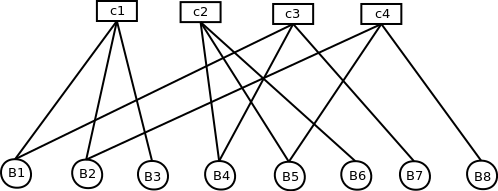
\includegraphics[height=4.5cm,width=10cm]{minSum1}
\caption[Tanner graph]{Tanner graph}
\end{figure}

\subsection{Sum Product Decoding\cite{9}}

The input bit probabilities are called the a priori probabilities.
The bit probabilities returned by the decoder are called the a posteriori probabilities.
For sum-product decoding these probabilities are expressed
as log-likelihood ratios (LLR).
\begin{align} L(x)=log\dfrac{p(x=0)}{p(x=1)}=log\dfrac{1-p(x=1)}{p(x=1)} \end{align}
 If p(x = 0) $>$ p(x = 1) then L(x) is positive.
%The greater the difference between p(x = 0) and p(x = 1), i.e. the more
%sure we are that p(x) = 0, the larger the positive value for L(x), and vic. versa.
%Log Likelihood Ratios are used to represent the metrics for a binary variable x
%by a single value rather than individual probability of being zero and one.
%The sign of L(x) provides the hard decision on x and the magnitude $|L(x)|$ represents
%the reliability of this decision.\\
%LLR based representation has benefit when probabilities
%Rneed to be multiplied LLR need only be added, reducing the implementation complexity.
T%he goal is to achieve maximum a posteriori probability of for each bit. 
The extra information about bit i received
from the parity-check j is called extrinsic information for bit i denoted by $E_{j,i}$. The probability ($P_{j,i}^{ext}$ ) that check j is satisfied when ith bit is one is equal to the probability of having odd number of 1s in the check j other than bit i.
\begin{align} P_{j,i}^{ext} = \dfrac{1}{2}-\dfrac{1}{2} \prod_{i'\in B_j, \ i'\neq i }(1-2P_{i'}^{int})  \end{align}
$P_{i'}^{int}$ is a priori probability of ith bit to be 1. Thus,
\[ E_{(j,i)} =  LLR (P_{j,i}^{ext}) = log \left(
\dfrac{1-P_{j,i}^{ext}}{P_{j,i}^{ext}} 
\right)
\]
\[ E_{(j,i)} = log
\left(
\dfrac{\dfrac{1}{2}+\dfrac{1}{2} \prod_{i'\in B_j \ i'\neq i }(1-2P_{i'}^{int}) }{\dfrac{1}{2}-\dfrac{1}{2} \prod_{i'\in B_j \ i'\neq i }(1-2P_{i'}^{int}) } 
\right)
 \]
Using relationship: $tanh \left(  \dfrac{1}{2}log \left( \dfrac{1-p}{p} \right) \right)=1-2p$;
\[ E_{(j,i)} = log
\left(
\dfrac{\dfrac{1}{2}+\dfrac{1}{2} \prod_{i'\in B_j \ i'\neq i }tanh(M_{j,i'}/2) }{\dfrac{1}{2}-\dfrac{1}{2} \prod_{i'\in B_j \ i'\neq i }tanh(M_{j,i'}/2) } 
\right)
 \]
where 
\[ M_{(j,i')} =  LLR (P_{j,i'}^{int}) = log \left(
\dfrac{1-P_{j,i'}^{int}}{P_{j,i'}^{int}} 
\right)
\]
Alternatively, using the relationship
\[ 2tan^{-1}(p)=log \left( \dfrac{1+p}{1-p} \right) \]
%%%%%%%%%%%%%%%%%%%%%%%%%%%%%%%%%%%%%%%%%%%%%
Thus extrinsic information from check j to bit i is:
\begin{align} E_{(j,i)} = 2tan^{-1} \left( \prod_{i'\in B_j ,\ i'\neq i }tanh(M_{j,i'}/2) \right) \end{align}
Total LLR passed to bit i is
\begin{align} L_i = LLR(P_i^{int}) = r_i + \sum_{j\in A_i} E_{j,i} \end{align}
where $r_i$ is input a priori for bit i.
But, message sent again from bit to check avoid the information which checks already have. Thus,
$M_{j,i}$ is not exactly the extrinsic information, it exclude the message generated by the same check node.\\
\begin{align}  M_{j,i} = \sum_{j'\in A_i j'\neq j} E_{j,i} + r_i \end{align}.\\
%\item %Each bit has access to the input a priori LLR, ri, and the LLRs from every
%connected check node. The total LLR of the i-th bit is the sum of these LLRs
     

After every iteration hard decision is made on the LLR post priori. If code satisfies $Hc^T=0$ then decoding stop else $M_{j,i}$ is found and next iteration is performed.
\subsection{Min Sum Decoding}
The min sum decode algorithm is simplification in the sum product algorithm. \\
For BPSK modulation transmitted $0's$ are represented as $-1s$ and transmitted $1s$ are represented as $1s$. \\
The probability that bit 1 is received 
\begin{align} f_y(y|f=-1) = \dfrac{1}{\sqrt{2\pi\sigma^{2}}} \exp{\dfrac{-(y+1)^2}{2\sigma^2}}
 \end{align}
 

The probability that bit 0 is received 
\begin{align} f_y(y|f=1) = \dfrac{1}{\sqrt{2\pi\sigma^{2}}} \exp{\dfrac{-(y-1)^2}{2\sigma^2}}
 \end{align}
 
Thus getting LLR as:
\begin{align}  LLR = \log\dfrac{f_y(y|f=-1)}{f_y(y|f=1)} = \dfrac{-2y}{\sigma^2}
 \end{align}
 
A priori information on the bit node side is expressed in term of LLR as: 
\begin{align}  aPriori[I] = -4 * C[I] * R * \dfrac{Eb}{No} 
 \end{align}
where C[I] = $i^{th}$ code block, R = code rate and 
$\dfrac{Eb}{No}$ = signal to noise power ratio\\
	
Messages are the information propagating from bit nodes to check nodes.
These are initialized to a priori of their respective bit node.	
\begin{align} message[I][J] = aPriori[I] 
 \end{align}
 
Extrinsic information of a bit node is calculated min sum of all the messages connected to 
	that particular check node. 
\begin{align} |E_{(j,i)}| =  Min_{i'\in B_j \ i'\neq i }|M_{j,i'}|   
 \end{align}

\begin{align} sign({E_{(j,i)}}) =  \prod_{i'\in B_j \ i'\neq i }sign(M_{j,i'})   
 \end{align}
 
A posteriori probabilities are the output bit probabilities.
These are used to modify the code block after every iteration.

\begin{align}  aPosteriori[I] = \sum_{j\in A_i} E_{j,i} + aPriori[I] 
 \end{align}
	
Then hard decision is taken on the a posteriori information, that represent the decoded code block.
If decoded code block satisfies $c*H^{T} = 0 $, then decoding stops. Else messages are updated and transmitted back to start the next iteration of decoding.
\begin{align}   message_{(j,i)} = aPosteriori[i] - E_{(j,i)}  
 \end{align}	



%   .
%   .
%   .

\appendix % Cue to tell LaTeX that the following 'chapters' are Appendices

% Import the Appendices
% \input{AppendixA}

\backmatter

% This file contains the templates for the last few pages of the thesis including 
% 1. List of publications
% 2. Acknowledgements

\newcommand{\publications}{

% Page number at bottom
\thispagestyle{plain}

% Title
\begin{center}{\huge{\textbf{List of Publications}} \par}\end{center}

\vspace*{15px}

% List your publications here

1.

2.
}

\newcommand{\acknowledgements}{

% Page number at bottom
\thispagestyle{plain}

% Title
\begin{center}{\huge{\textit{Acknowledgements}} \par}\end{center}

\vspace*{15px}

% Write acknowledgement here

\noindent I would like to thank ...

\vspace*{15px}

\begin{flushright}
{Signature: ......................................\\[0.4cm]}

{\textbf{\authorName}\\[0.0cm]\rollNo\\[2.0cm]}
\end{flushright}

\begin{flushleft}
{Date:} ...... \currentmonth { } \currentyear\\
\end{flushleft}
}




% Bibliography

\label{Bibliography}
\lhead{\emph{Bibliography}}

\bibliographystyle{unsrtnat} % Use the "unsrtnat" BibTeX style for formatting the Bibliography

\bibliography{Bibliography} % The references (bibliography) information are stored in the file named "Bibliography.bib"

\clearpage

% List of Publications
\addcontentsline{toc}{chapter}{List of Publications}
\publications

\clearpage

% Acknowledgements
\addcontentsline{toc}{chapter}{Acknowledgements}
\acknowledgements


\end{document}
% End of the document
